\documentclass[12pt]{article}
\usepackage{graphicx}
\usepackage{amsmath}
\usepackage{multicol}
\usepackage[right=1in,left=1in,top=1in,bottom=1in]{geometry}
\DeclareGraphicsExtensions{.pdf,.png,.jpg,.eps}
\graphicspath{'/Users/Mitch/Dropbox/Adv\ Lab/Lab\ 2/Data/Figures/'}

\begin{document}

\begin{center}
\textbf{Integration and Random Numbers} \\ 
Mitchell Miller \\
Illinois Institute of Technology \\
March  27 2012 {\ \\ \ \\}
\textbf{Abstract}\\
\end{center}
\noindent
The ability to integrate complex functions numerically is an incredibly valuable skill for any physicist.  In this lab three methods of integration were explored:  Romberg, Gaussian Quadrature, and Monte Carlo simulations.  The Romberg method was used to extrapolate the approximations obtained via Simpson's Rule to achieve highly accurate results.  Two types of Quadrature methods were employed to find exact results for both single and multi-dimensional integrals.  Finally, Monte Carlo simulations were used to quickly calculate high dimensional integrals.
\pagebreak
\section{Introduction}
\subsection{Romberg Integration}
The Romberg method begins with a series of approximations obtained via the trapezoidal rule.  The trapezoidal rule is a geometric approximation for the area beneath a function, $f(x)$, approximating the total area as a sum of the area contained by many, discrete trapezoids.    
\begin{equation}
\label{trap}
\int_{x_0}^{x_n} \! f(x) \, \mathrm{d} x \approx h (\frac{f_0}{2} + f_1+f_2+...+f_{n-1}+\frac{f_n}{2})
\end{equation}
The approximation with $n=2^m$ is defined as $T_{m,0}$ and the error is known to be of order $h^2$.  One can then obtain $T_{m+1,0}$ by using a step size, $h/2$, half that of the previous approximation.    The error of this new term is one quarter of the previous.  One can then combine these two terms to find a new approximation, $T_{m+1,1}$, with the leading error term eliminated.
\begin{equation}
\label{T11}
T_{m+1,1} = \frac{4T_{m+1,0}-T_{m,0}}{3}
\end{equation}
This new approximation has had the leading error term, proportional to $h^2$, eliminated; however, now the next term, $O(h^4)$, dominates.  If the step size is halved again, one obtains $T_{m+2,1}$, which has one sixteenth the error of the previous approximation.  Now, this error can be eliminated in a similar fashion described above.
\begin{equation}
\label{T22}
T_{m+2,2} = \frac{16T_{m+2,1}-T_{m+1,1}}{15}
\end{equation}
With this recursive relation, one can build a triangular array of approximations with increasingly accurate elements.  Careful examination of \eqref{T11} and \eqref{T22} will reveal that a general element in this matrix can be calculated as
\begin{equation}
\label{Tkk}
T_{m+k,k} = \frac{4^kT_{m+k,k-1}-T_{m+k-1,k-1}}{4^k-1}
\end{equation}
It is important to consider the cases in which Romberg integration is not a useful approximation.  When considering functions that have undefined derivatives at the integration range's endpoints, the Romberg method can produce highly inaccurate results.  To avoid this, one can perform the 'Ratio Test.'  By considering the difference between three subsequent steps, one can obtain a fraction which should always result in 4.
 \begin{equation}
\label{Rm}
R_m = \frac{T_{m-1,0}-T_{m,0}}{T_{m,0}-T_{m+1,0}} \approx 4
\end{equation}
If this test results in a value not near 4, one can attempt a change of variables to eliminate the undefined derivatives.  
\subsection{Gaussian Quadrature}
The Gaussian Quadrature method approximates the integral of a function, $f(x)$, as a sum of the function's values multiplied by a weighting function at $N$ discrete points.
\begin{equation}
\label{GaussLeg}
\int_{a}^{b} \! f(x) \, \mathrm{d} x \approx \sum_{m=0}^N W_mf(x_m))
\end{equation}
One should note that, at this point, both $W_m$ and $x_m$ are unknown, giving $2N$ values to be found.  To find these coefficients, this approximation can be required to be exact for all polynomials, $f(x)$, of order $2N-1$ and below.  Now, a new function, $\phi(x)$, is defined which is orthogonal to $f(x)$ with respect to $W$.  Now, $f(x)$ can be re-expressed as a product
\begin{equation}
\label{fLeg}
f(x) = q_{N-1}(x)\phi_N(x)+r_{N-1}(x)
\end{equation}
where $q_{N-1}(x)$ and $r_{N-1}(x)$ are both of order $N-1$.  Because $\phi_m$ is a complete set of functions, $q_{N-1}$ can be expanded as the following
\begin{equation}
\label{qLeg}
q_{N-1}(x)=\sum_{i=0}^{N-1}q_i\phi_i(x)
\end{equation}
For the given orthogonality conditions to be true, it is found that the only valid $x_m$ values are the zeros of $\phi(x)$.  Making the requirement that $W(x)=1$ and finite limits of integration, it is found that these $x$ values must be the zeroes of the Legendre polynomials.  Finally, one can find that the individual weights at these $x_m$ are
\begin{equation}
\label{Wm}
W_m=\int_a^b l_{i,N}(x_m) \mathrm{d}x
\end{equation}
Where $l_{i,N}(x)$ is Lagrange's interpolating polynomial discussed in the previous lab. \\
This method is useful when the bounds of integration are finite, but if one hopes to perform an integral with boundaries at infinity, several changes must be made.  First, one must convert the integrating function into the following form
\begin{equation}
\label{GausExpo}
g(x) = e^{-x}f(x)
\end{equation}
Evaluating the integral
\begin{equation}
\label{LagInt}
\int_0^{\infty} g(x) \mathrm{d}x = \sum_{m=1}^N W_m f(x_m)
\end{equation}
one finds that the values for $x_m$ in order to meet the orthogonality conditions, as described above, are the zeroes of the Laguerre polynomials.
\subsection{Monte Carlo}
Monte Carlo integration makes use of random number generators and a very large sample size to generate an average of a function, $f(x)$, over the integration range.  This average is then multiplied by the width of the range to obtain the area contained beneath the curve
\begin{equation}
\label{MonteInt}
\int_a^b f(x) \mathrm{d}x \approx (b-a) \frac{1}{N}\sum_{i=1}^N f(x_i)
\end{equation}
where $x_i$ are a series of uniformly distributed random values between $a$ and $b$.  Since all that is necessary for the evaluation of this technique is a calculation of the function, it is a very fast method.  One can easily calculate a million random values, providing a high degree of accuracy, in a very short amount of time.


If the accuracy is not enough using purely random points, a technique called importance sampling can be implemented.  Importance sampling takes points that contribute more heavily to the average of the function.  Given a function, $f(x)$, a second function, $g(x)$, can be chosen such that $f(x) \approx g(x)$.  Thus
\begin{equation}
\label{Import}
\int_a^b f(x) \mathrm{d}x = \int_a^b \frac{f(x)}{g(x)} g(x) \mathrm{d}x = \int_{y^{-1}(a)}^{y^{-1}(b)}  \frac{f(x)}{g(x)} \mathrm{d}x
\end{equation}
where
\begin{equation}
\label{ImportY}
y(x) = \int^x g(t) \mathrm{d}t 
\end{equation}
If $g(x)$ is a sufficiently good approximation of $f(x)$, then \eqref{Import} becomes an integral of 1 and the integral is sampled uniformly over $y(x)$.  This will cause the random numbers to be generated more heavily in the regions where the function is large.


Since Monte Carlo integration uses random numbers, it is ruled by standard probability laws.  If one were to calculate the same integral 100 times, it is very likely that the output would be different every time and none of the results would be the exact answer.  If one plots the different values obtained through Monte Carlo integration versus the number of times that value occurs, a Gaussian distribution is obtained.  This distribution has a spread proportional to $\frac{1}{\sqrt{N}}$, where $N$ is the number of trials.  Using probability theory, one can find the exact expression for the standard deviation as
\begin{equation}
\label{StDev}
\sigma_N = \sqrt{\frac{\frac{1}{N}\sum_i f(x_i)^2-(\frac{1}{N} \sum_i f(x_i))^2}{N-1}}
\end{equation}
This allows \eqref{MonteInt} to be rewritten as
\begin{equation}
\label{MonteIntSigma}
\int_a^b f(x) \mathrm{d}x \approx (b-a) (<f(x)>_N \pm \sigma_N)
\end{equation}
with a 68.3\% confidence where $<f(x)>$ is the average value of the function, $f(x)$.
\section{Applications}
\subsection{Romberg Integration}
The first test of the Romberg method described above was the exploration of 'knife edge' diffraction.  This is the diffraction of light around a perfectly flat surface.  The intensity of light as the distance from the edge changes is described as
\begin{equation}
\label{DiffInten}
I=\frac{1}{2}I_0 [ [C(v) + \frac{1}{2}]^2 + [S(v) + \frac{1}{2}]^2]
\end{equation}
where $C(v)$ and $S(v)$ are the Fresnel integrals
\begin{equation}
\label{CFres}
C(v) = \int_0^v \mathrm{cos}(\frac{\pi\omega^2}{2}) \mathrm{d}\omega
\end{equation}
\begin{equation}
\label{SFres}
S(v) = \int_0^v \mathrm{sin}(\frac{\pi\omega^2}{2}) \mathrm{d}\omega
\end{equation}
Using Romberg integration, \eqref{DiffInten} was evaluated to generate the diffraction pattern one would observe.  It is shown in 
\begin{figure}[!h]
\centering
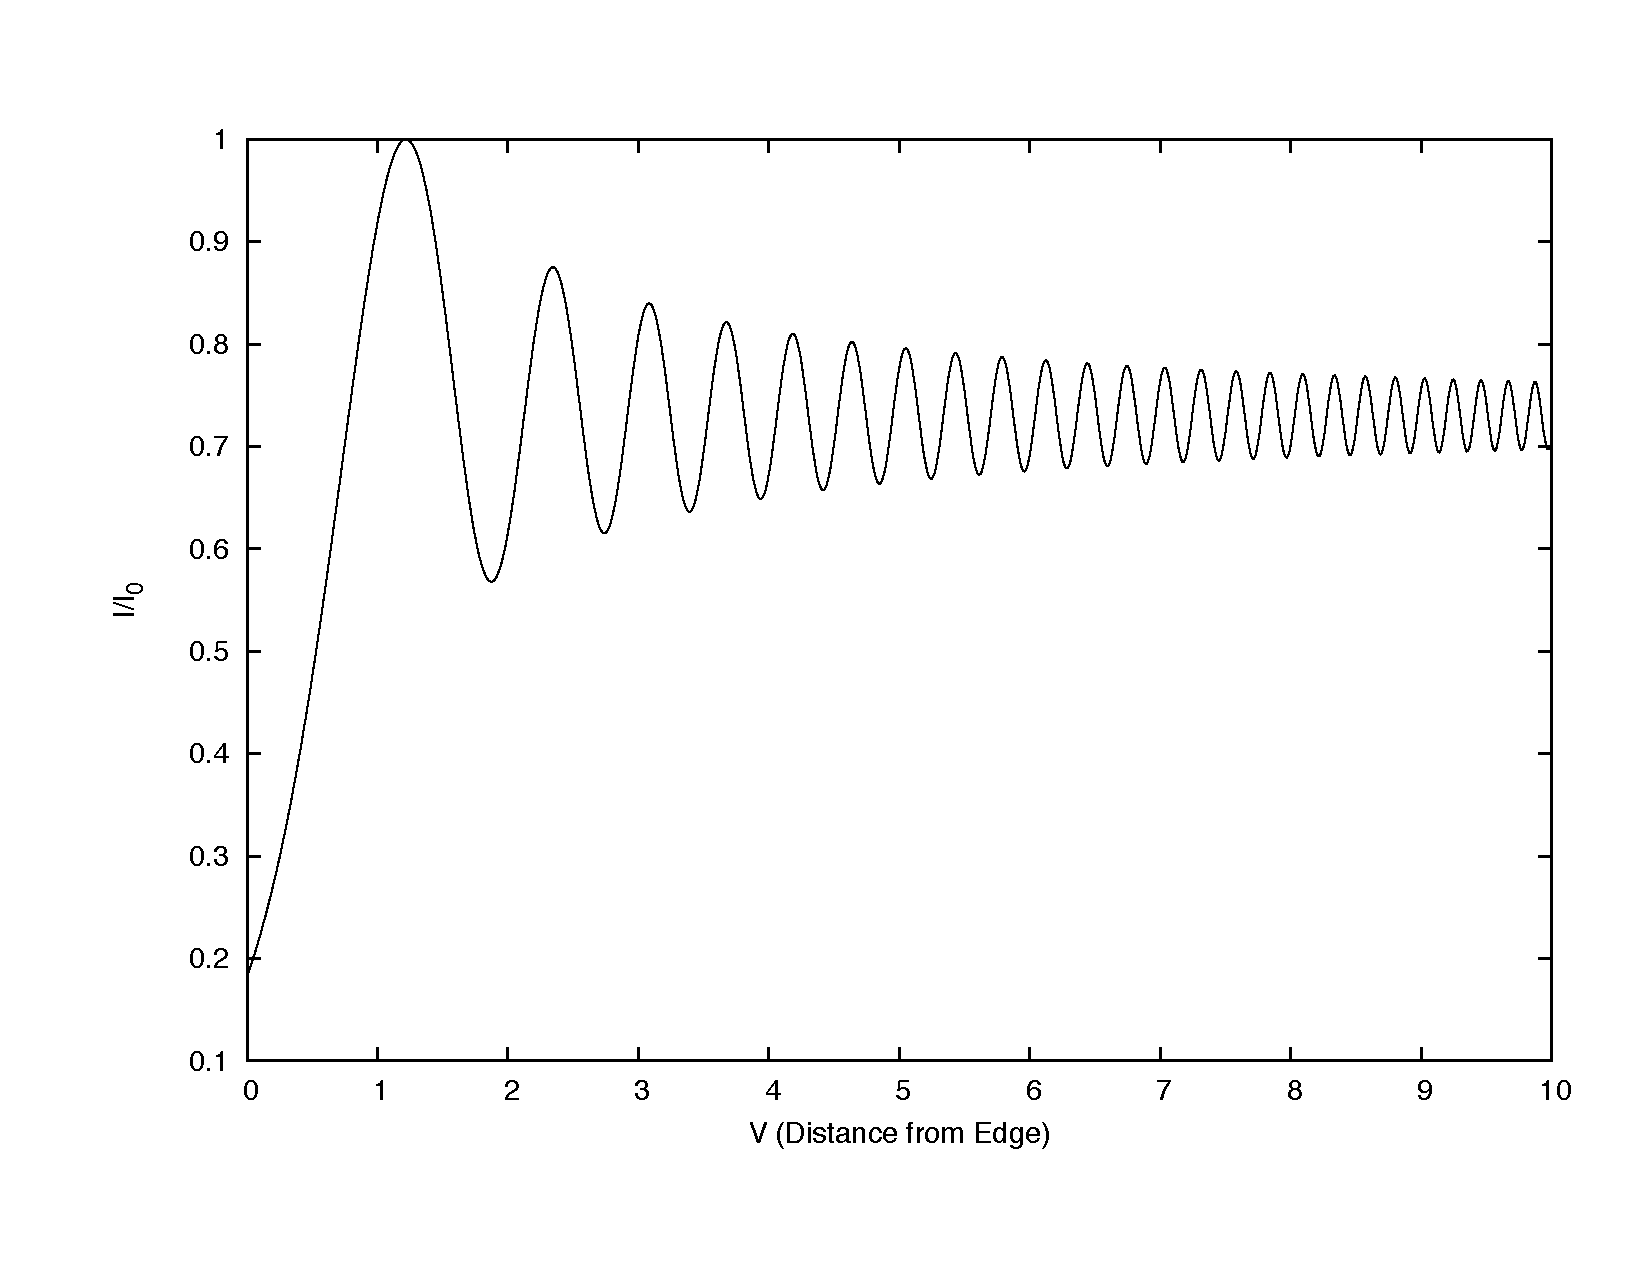
\includegraphics[width =120 mm, height = 75mm]{Ex_4_4.pdf}
\caption{A plot of relative intensity versus distance from edge.}
\label{fig:DiffInten}
\end{figure}
Figure \ref{fig:DiffInten} that, as the distance from the edge increases, there are oscillations in intensity.  This is the standard result of optical diffraction.  However, this is one important feature:  the intensity does not converge to zero, but at some finite value, approximately $0.73$.

Now consider a function that tests the inadequacies of the Romberg method.
\begin{equation}
\label{Test}
I = \int_{-1}^1 \sqrt{(1-x^2)(2-1)} \mathrm{d}x
\end{equation}
This is the equation shown in Fig. \ref{fig:45}.  At the endpoints, $-1$ and $1$, the derivative is infinite.  Using this form of the integrand, the following results were obtained with Romberg integration.
\begin{figure}[!h]
\centering
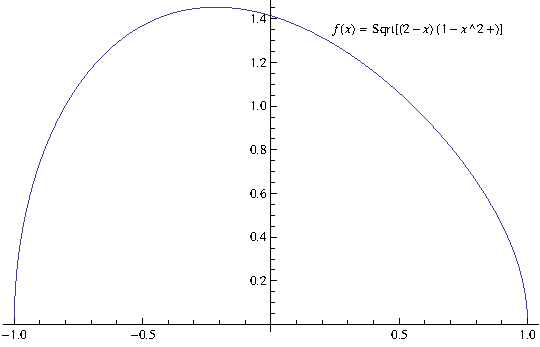
\includegraphics[width =120 mm, height = 75mm]{Ex_4_5.pdf}
\caption{A plot of \eqref{Test}.}
\label{fig:45}
\end{figure}
\begin{center}
Table 1:  Romberg Integration \\
\begin{tabular}{ | c | c | c | c | c | c |}
\hline
m& $T_{m,0}$ & $T_{m,1}$ & $T_{m,2}$ & $T_{m,3}$ & $R_m$ \\ \hline
1&	1.414214&	1.885618&	&	&	2.784562\\ \hline
2&	1.922090&	2.091382&	2.105100&	&	2.800385\\ \hline
3&	2.103450&	2.163903&	2.168737&	2.169748&	2.812189\\ \hline
4&	2.167940&	2.189437&	2.191139&	2.191495&	2.819640\\ \hline
5&	2.190812&	2.198436&	2.199036&	2.199161&	2.823852\\ \hline
6&	2.198911&	2.201611&	2.201823&	2.201867&	2.826093\\ \hline
7&	2.201777&	2.202733&	2.202808&	2.202823&	2.827248\\ \hline
8&	2.202791&	2.203129&	2.203155&	2.203161&	2.827835\\ \hline
9&	2.203150&	2.203269&	2.203278&	2.203280&	2.827835\\ \hline
\end{tabular}
\end{center}
The exact solution to \eqref{Test} is $2.20334573182474$.  Although this answer is achieved via the Romberg method in its original form, the ratio test fails and the answer lacks accuracy beyond the third decimal, and many steps are required.  By making a change of variables, $x = \mathrm{cos}(\theta)$, \eqref{Test} can be rewritten as
\begin{equation}
\label{TestRe}
I = \int_0^\pi \mathrm{sin}^2\theta\sqrt{2-\mathrm{cos}\theta} \mathrm{d}x
\end{equation}
which is well behaved at the endpoints.
\begin{center}
Table 2:  Romberg Integration (Alternate Form) \\
\begin{tabular}{ | c | c | c | c | c | }
\hline
m& $T_{m,0}$ & $T_{m,1}$ & $T_{m,2}$ & $T_{m,3}$ \\ \hline
1&	2.221441469079180&	2.961921958772240&	&	\\ \hline
2&	2.203360140807090&	2.197333031383061&	2.146360436223782&	\\ \hline
3&	2.203345731924877&	2.203340928964139&	2.203741455469544&	2.204652265298842\\ \hline
4&	2.203345731824744&	2.203345731791366&	2.203346051979848&	2.203339775733979\\ \hline
5&	2.203345731824744&	2.203345731824744&	2.203345731826969&	2.203345726745177\\ \hline
6&	2.203345731824744&	2.203345731824744&	2.203345731824743&	2.203345731824708\\ \hline
7&	2.203345731824744&	2.203345731824744&	2.203345731824744&	2.203345731824744\\ \hline
8&	2.203345731824744&	2.203345731824744&	2.203345731824744&	2.203345731824744\\ \hline
9&	2.203345731824743&	2.203345731824743&	2.203345731824743&	2.203345731824743\\ \hline
\end{tabular}
\end{center}
Using this form of the integral, the Romberg method converges almost immediately.  The convergence occurs so quickly that implementation of the ratio test is not helpful because the denominator quickly converges to $0$, resulting in an indeterminate ratio.

The final application of the Romberg method is the analysis of the simple pendulum.  This application seeks to find the period of the pendulum which is given as
\begin{equation}
\label{period}
T = 4\sqrt{\frac{l}{2g}} \int_0^{\theta_0} \frac{\mathrm{d}\theta}{\sqrt{\mathrm{cos} \theta - \mathrm{cos} \theta_0}}
\end{equation}
Since this integral is indeterminate at the boundary $\theta_0$, some substitutions must be made.  After completing these substations, a new expression is found.
\begin{equation}
\label{periodK}
T = 4\sqrt{\frac{l}{g}} \mathrm{K}(\mathrm{sin}\frac{\theta_0}{2})
\end{equation}
where $K(x)$ is
\begin{equation}
\label{K}
K(k) = \int_0^{\frac{\pi}{2}} \frac{\mathrm{d}\zeta}{\sqrt{1-k^2\mathrm{sin}^2\zeta}}
\end{equation}
Solving for the period of a pendulum analytically, using the small angle approximation, one finds that the period is approximately $2\pi\sqrt{\frac{l}{g}}$.  Using Romberg integration and incrementing the starting amplitude, one finds that at $\theta_0$ greater than $22.5^\circ$, the approximation is off by more than 1\%.
\begin{figure}[!h]
\centering
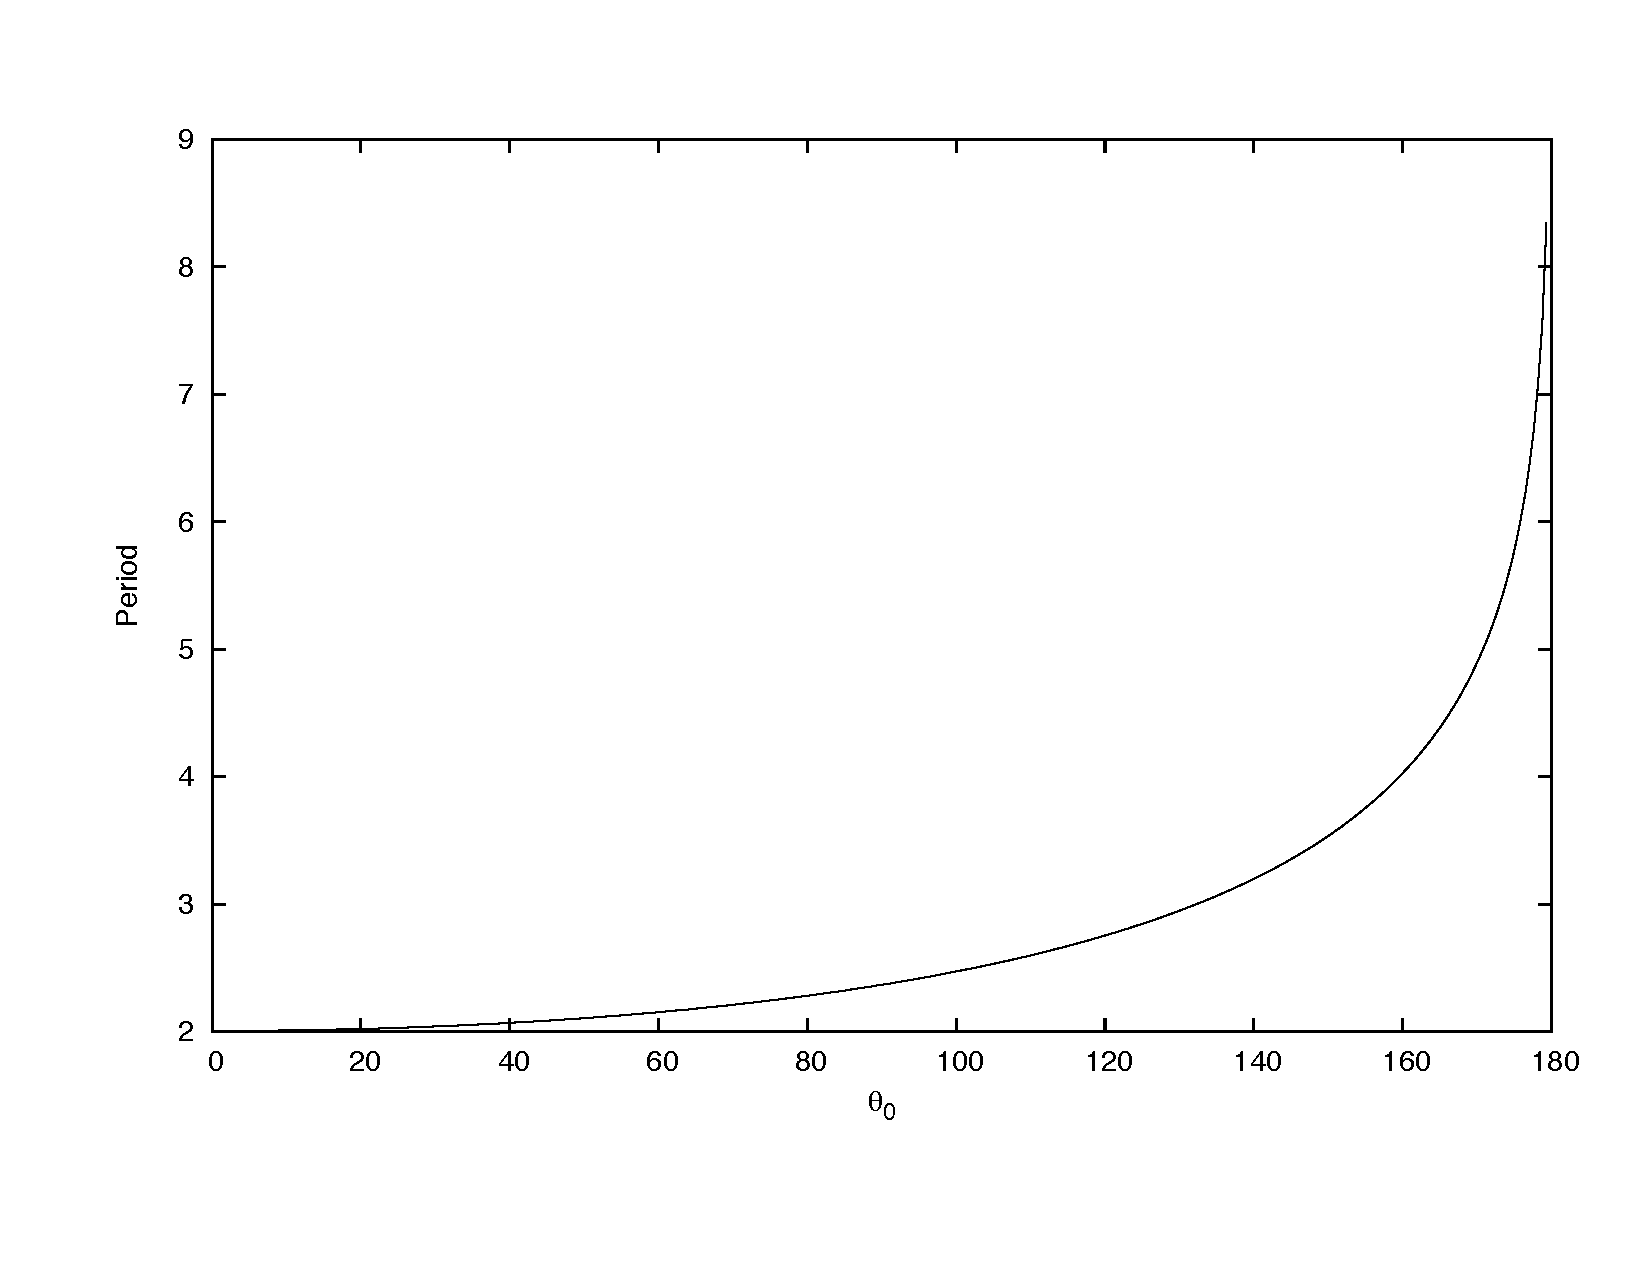
\includegraphics[width =120 mm, height = 75mm]{Ex_4_6.pdf}
\caption{A plot of initial angle of pendulum and the period.}
\label{fig:46}
\end{figure}
Figure \ref{fig:46} shows the period versus the initial angular displacement of the pendulum.  It is clear at $180^\circ$ that the period diverges to infinity.  This corresponds to the unstable equilibrium position at which the pendulum sits perfectly vertically, and thus has a period of infinity.
\subsection{Gaussian Quadrature}
To begin the exploration of Gaussian Quadrature integration, several simple function were explored.  First, a simple polynomial was integrated.
\begin{equation}
\label{x7}
I = \int_0^1 x^7 \mathrm{d}x
\end{equation}
\begin{figure}[!h]
\centering
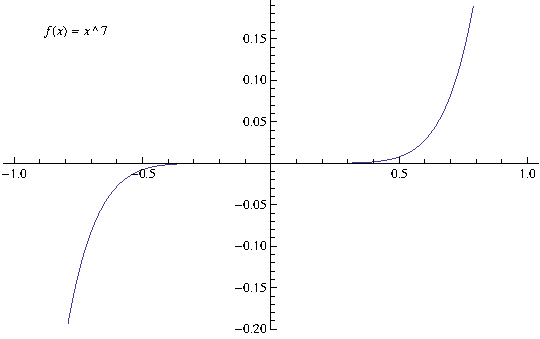
\includegraphics[width =120 mm, height = 75mm]{Ex_4_15.pdf}
\caption{A plot of the integrand of \eqref{x7}.}
\label{fig:415}
\end{figure}
This integral can be solved very quickly to find $I=\frac{1}{8}=0.125$.  The Gaussian Quadrature method using the Legendre polynomial zeroes outputs the results shown in Table 3.
\begin{center}
Table 3:  Gaussian Quadrature Integration of \eqref{x7} \\
\begin{tabular}{ | c | c |}
\hline
N & Integration Result \\ \hline
2&	0.094907407407407 \\ \hline
3&	0.123750000000000 \\ \hline
4&	0.125000000000000 \\ \hline
5&	0.125000000000000 \\ \hline
\end{tabular}
\end{center}
Since the polynomial is seventh order, an exact answer is obtain at any N greater than 3.  This is confirmed by the data in Table 3.

Next, a more complicated function was evaluated, a Gaussian distribution.
\begin{equation}
\label{GaussDist}
I = \int_0^1 e^{-x^2} \mathrm{d}x
\end{equation}
Since this is not a polynomial, Gaussian Quadrature integration will never find an exact solution.  However, as N is increased, the output gets closer and closer to the exact solution, 0.746824132812427.
\begin{center}
Table 4:  Gaussian Quadrature Integration of \eqref{GaussDist} \\
\begin{tabular}{ | c | c |}
\hline
N & Integration Result \\ \hline
2&	0.746594688282859\\ \hline
3&	0.746814584191256\\ \hline
4&	0.746824468130994\\ \hline
5&	0.746824126766248\\ \hline
\end{tabular}
\end{center}
At $N=5$, this integration yields results accurate to the sixth decimal place.  

Now consider an integral that requires the use of the Laguerre polynomials.
\begin{equation}
\label{418}
I = \int_0^\infty \frac{x^3}{e^x-1} \mathrm{d}x
\end{equation}
This integral has an exact solution of 6.49393940226683.
\begin{center}
Table 4:  Gaussian Quadrature Integration of \eqref{418} \\
\begin{tabular}{ | c | c |}
\hline
N & Integration Result \\ \hline
2&	6.413727469517580\\ \hline
4&	6.494535639802627\\ \hline
6&	6.493941414321218\\ \hline
8&	6.493935665619213\\ \hline
\end{tabular}
\end{center}
Again, no value of N provides an exact solution, but at $N=8$, the approximation is accurate to 5 decimal points.

Next, multidimensional integration was explored.  First, a simple exponential was evaluated
\begin{equation}
\label{2DInt}
I = \int_0^1\int_0^2 e^{-xy} \mathrm{d}x \mathrm{d}y
\end{equation}
This integral has a solution of $I = 1.31926335616954$.  Using Gaussian Quadrature with $N=5$, an approximation of $I \approx 1.319263356109597$ was found.  This approximation is accurate to 10 decimal points.

The final application of Gaussian Quadrature integration is the analysis of a square, uniform charge distribution.  If one has a square charge distribution of side length 2 centered about the origin, the form for the potential at a point $(x_p,y_p)$ is given as 
\begin{equation}
\label{Potential}
\Phi(x_p,y_p) =\frac{\rho}{4\pi\epsilon_0} \int_{-1}^1\int_{-1}^1 \frac{\mathrm{d}x \mathrm{d}y}{\sqrt{(x-x_p)^2+(y-y_p)^2}}
\end{equation}
For the purposes of this lab, $\frac{\rho}{4\pi\epsilon_0}$ was taken to be equal to one.  A plot of a small range ($x_p$ and $y_p$ [2:20]) is shown in Figure \ref{fig:Potential}.
\begin{figure}[!h]
\centering
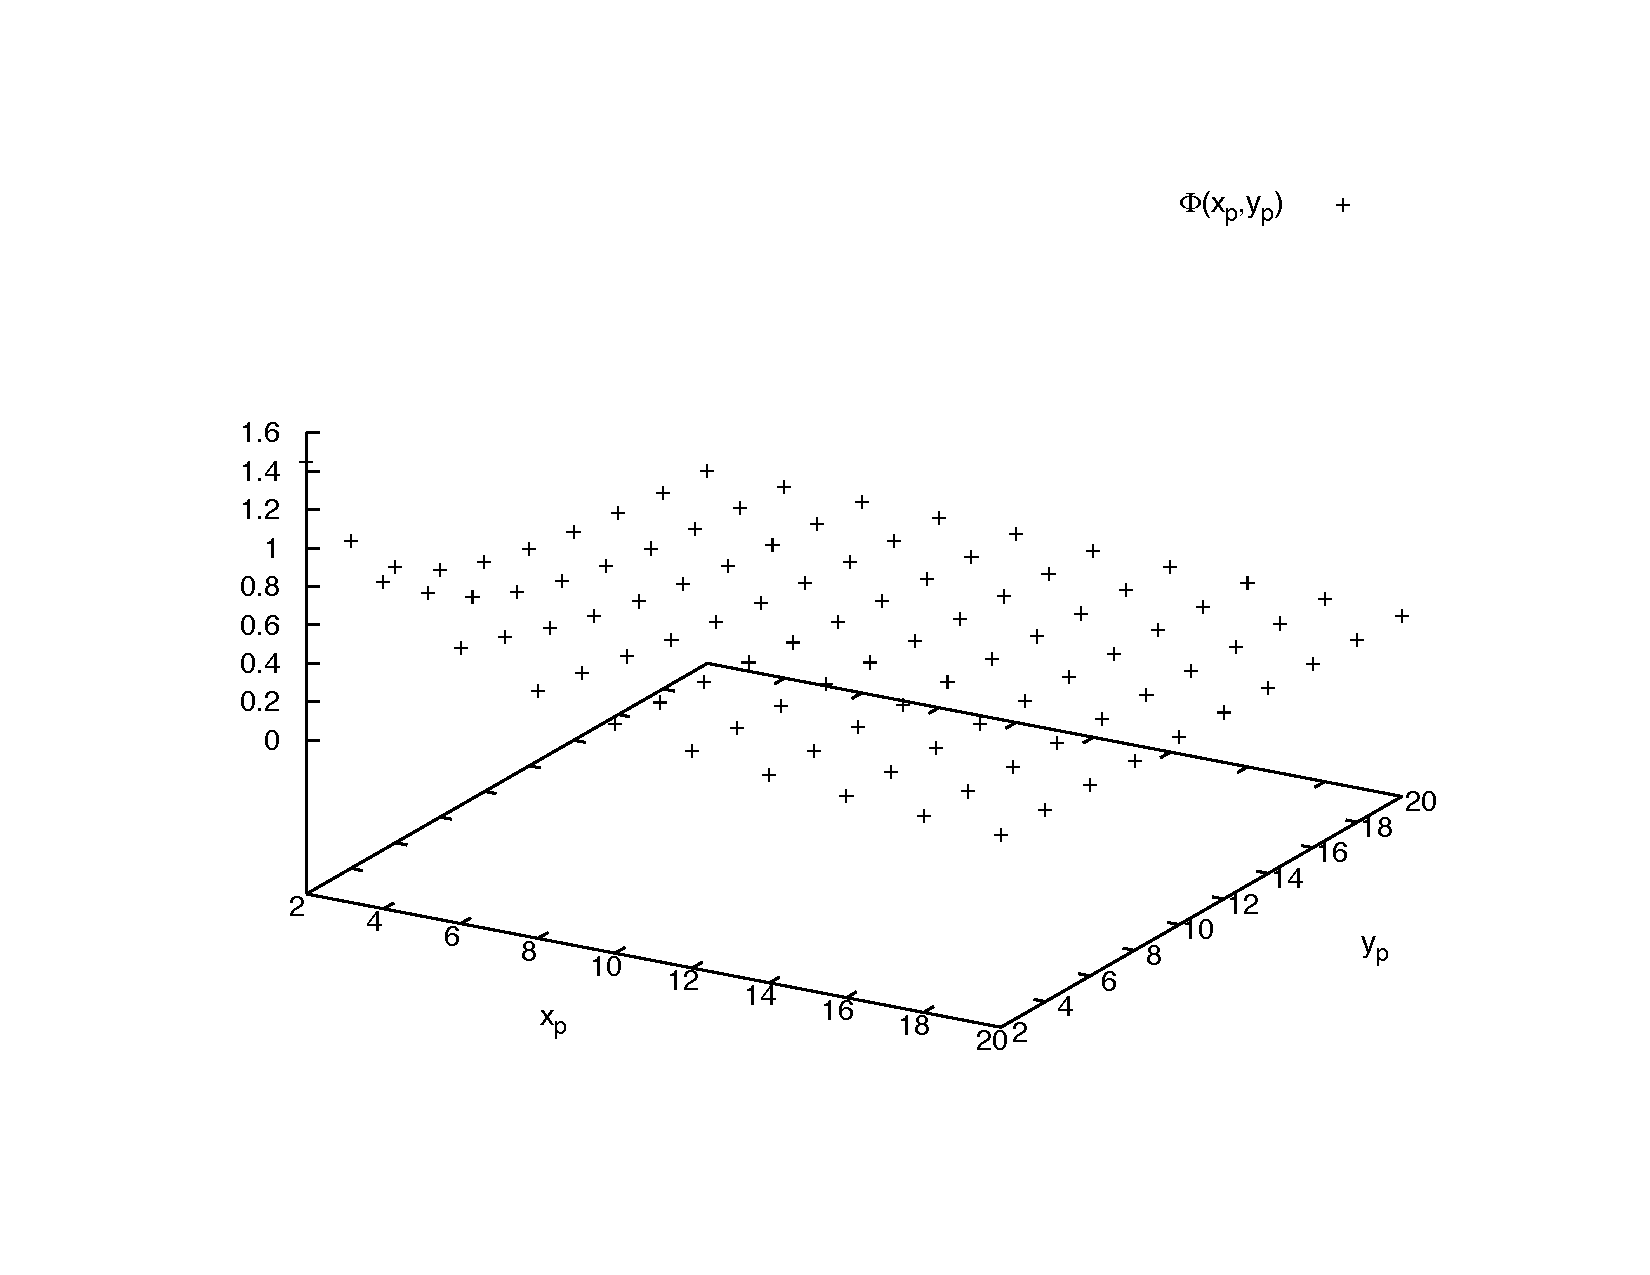
\includegraphics[width =120 mm, height = 75mm]{Ex_4_22.pdf}
\caption{A plot of potential versus distance from the origin.}
\label{fig:Potential}
\end{figure}
As expected, when the distance from the charge distribution is large, the potential approaches zero.

\subsection{Monte Carlo}
The first application of Monte Carlo integration was a demonstration of its statistical nature.  A very simple exponential integral was evaluated 10000 times.  
\begin{equation}
\label{ExpInt}
I = \int_0^1 e^x \mathrm{d} x
\end{equation}
First, \eqref{ExpInt} was evaluated using 100 random points.  This resulted in a distribution of solutions shown in Figure \ref{fig:Monte100}.
\begin{figure}[!h]
\centering
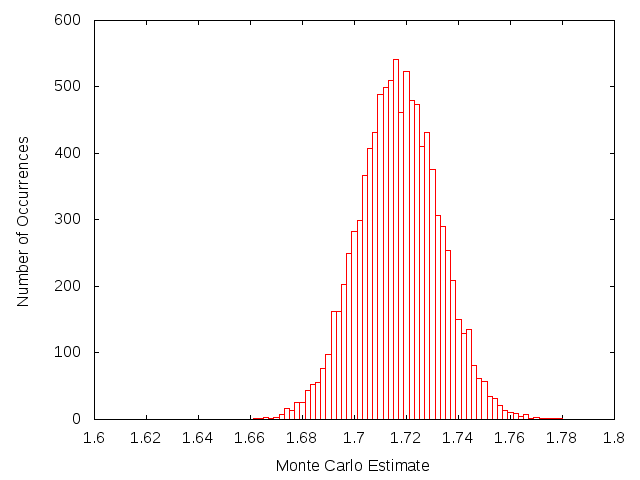
\includegraphics[width =120 mm, height = 70mm]{Fig_4_12_100.png}
\caption{A distribution of 10000 Monte Carlo evaluations of \eqref{ExpInt} using 100 points.}
\label{fig:Monte100}
\end{figure}
The same integral was then re-evaluated using 400 random points.
\begin{figure}[!h]
\centering
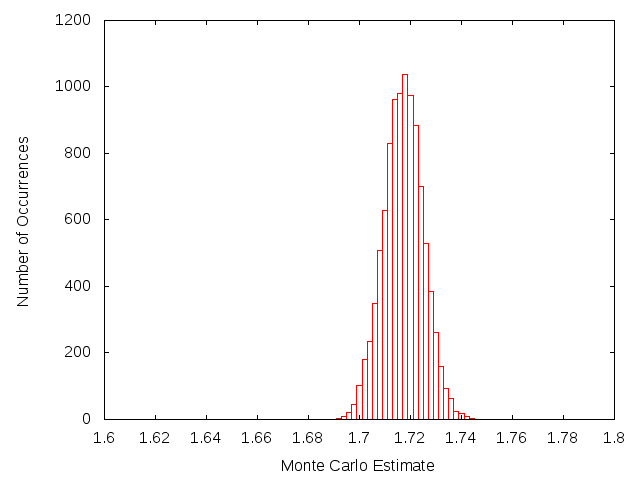
\includegraphics[width =120 mm, height = 70mm]{Fig_4_12_400.png}
\caption{A distribution of 10000 Monte Carlo evaluations of \eqref{ExpInt} using 400 points.}
\label{fig:Monte400}
\end{figure}
Both these distributions are centered about 1.718, the analytic solution to this integral, but they clearly have different standard deviations, as predicted by \eqref{StDev}.

The next demonstration of the statistical nature of Monte Carlo integration was the analysis of a simple sum
\begin{equation}
\label{Sum}
y = \sum_{i=1}^{12} r_i
\end{equation}
where $r_i$ is a random number between zero and one.  Since Monte Carlo techniques work by averaging a function using random numbers, one would expect this sum of twelve points between zero and one to have a result, on average, of 6.  
\begin{figure}[!h]
\centering
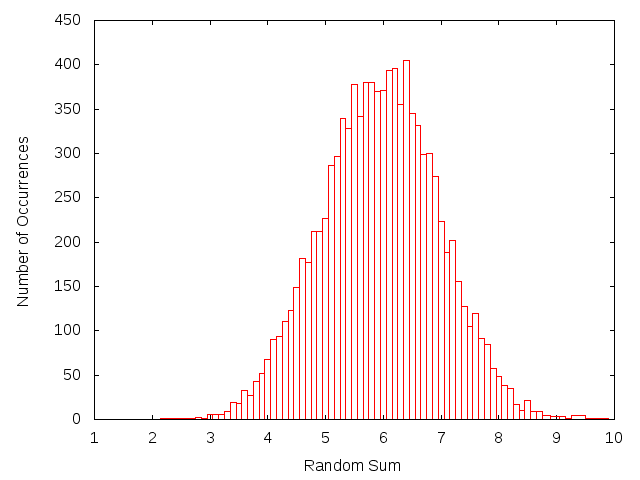
\includegraphics[width =120 mm, height = 70mm]{Ex_12_10.png}
\caption{A distribution of 10000 Monte Carlo evaluations of \eqref{Sum}.}
\label{fig:Monte6}
\end{figure}
Figure \ref{fig:Monte6} shows the distribution of 10000 evaluations of \eqref{Sum}.  This distribution is centered about 6, as expected.  

The final test of Monte Carlo integration was the analysis of the exchange energy of the first excited state of a helium atom.  To solve this problem, one begins with the Hamiltonain
\begin{equation}
\label{Ham}
H = \frac{P_1^2}{2m_e}+\frac{P_2^2}{2m_e}-Ze^2[\frac{1}{|r_1|}+\frac{1}{|r_2|}]+\frac{e^2}{|r_1-r_2|}
\end{equation}
where $P_i$ and $r_i$ are the momenta and radii of each electron, $e$ is the charge and $m_e$ is the mass of an electron.  Unfortunately, the dependence on $r_1-r_2$ makes this problem impossible to solve analytically.  There are several clever tricks one can implement to turn this into something that can be easily solved with pen and paper, however it is also possible to simply solve this problem numerically.

When helium is placed in its first excited state, one electron is promoted to $|2 l m>$.  In spectroscopic notation, this electron can occupy either the 2S or 2P states.  Since it is known that the total wave function is anti-symmetric, one can use first order perturbation theory to find the energy shift from coulombic interaction to be
\begin{equation}
\label{Ej}
\Delta E_j = e^2 \int \int |\psi_{100}(r_1)|^2 |\psi_{2lm}(r_2)|^2 \mathrm{d}^3r_1 \mathrm{d}^3r_2
\end{equation}
\begin{equation}
\label{Ek}
\Delta E_k = e^2 \int \int \psi^*_{100}(r_1) \psi^*_{2lm}(r_2)\frac{1}{|r_1-r_2|}\psi_{2lm}(r_2 \psi_{100}(r_1) \mathrm{d}^3r_1 \mathrm{d}^3r_2
\end{equation}
and the total energy shift is defined as
\begin{equation}
\label{DeltaE}
\Delta E = \Delta E_j \pm \Delta E_k = J \pm K
\end{equation}
From this, one can use Monte Carlo integration to perform the six dimensional integral necessary to calculate $J$ and $K$.

Both $J$ and $K$ can assume two different values, depending on the spin state.
\begin{equation}
\label{DeltaE2S}
\Delta E_{1s,2s} = J_{1s,2s} \pm K_{1s,2s} = 11.4 \mathrm{eV} \pm 1.2 \mathrm{eV}
\end{equation}
\begin{equation}
\label{DeltaE2P}
\Delta E_{1s,2p} = J_{1s,2p} \pm K_{1s,2p} = 13.2 \mathrm{eV} \pm 0.9 \mathrm{eV}
\end{equation}
These values were evaluated using Monte Carlo integration.  Each Cartesian component (x,y,z) for each of the two electrons were evaluated using the C random number function 'drand48().'  Each integral was evaluated using $10^7$ iterations and these integrals were averaged over $10^3$ trials.  
\begin{center}
Table 5:  Helium Atom Energy Shifts \\
\begin{tabular}{ | c | c | c|}
\hline
State&Energy (eV) &\% Error \\ \hline
$J_{1s,2s}$&	11.183847&1.89608 \\ \hline
$K_{1s,2s}$&	1.407396& 17.283\\ \hline
$J_{1s,2p}$&	19.072715&44.4903 \\ \hline
$K_{1s,2p}$&	0.870096&3.32267 \\ \hline
\end{tabular}
\end{center}
The average error of these values is 16.8 \%, however, the error from $J_{1s,2p}$ skews this value heavily.  It is likely that, since this value is the only major outlier, this error is simply a result of the random nature of the integration technique.  One could expect to improve the accuracy of these results with a higher number of iterations and trials.  However, the time required to perform these calculations is quite large, and the values generated from this simulation were sufficiently accurate to demonstrate proof of the technique for the purposes of this lab.

The final application of Monte Carlo techniques is the use of random numbers in simulations.  The Random Walk problem studies the behavior of a particle in some medium.  As this particle moves through the medium, it encounters scattering sites which cause it to change direction.  Using a random number generator to generate two angles ($\theta$ and $\phi$ in spherical coordinates), a random path is built using conservation of energy and momentum.  
\begin{figure}[!h]
\centering
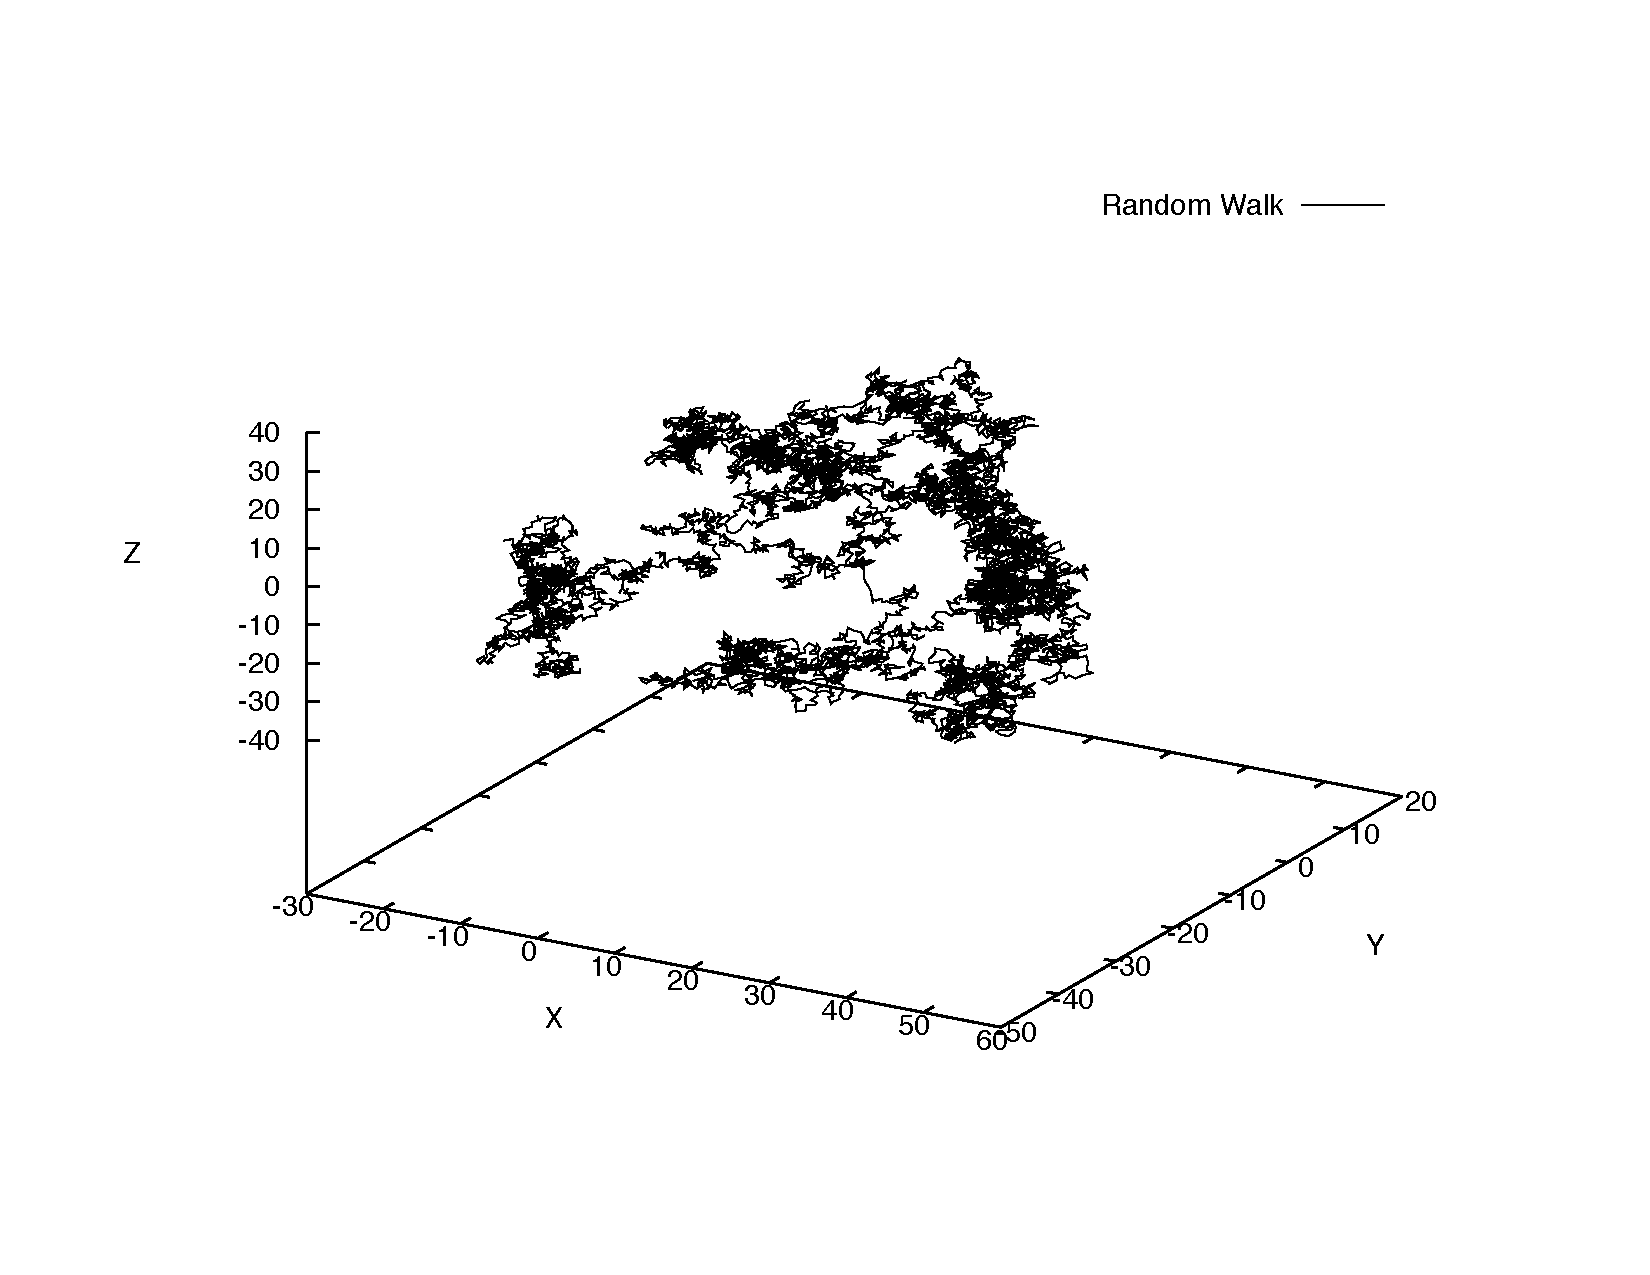
\includegraphics[width =120 mm, height = 90mm]{Ex_4_30.pdf}
\caption{10000 steps in a Monte Carlo simulation of the random walk problem.}
\label{fig:RandomWalk}
\end{figure}
\begin{figure}[!h]
\centering
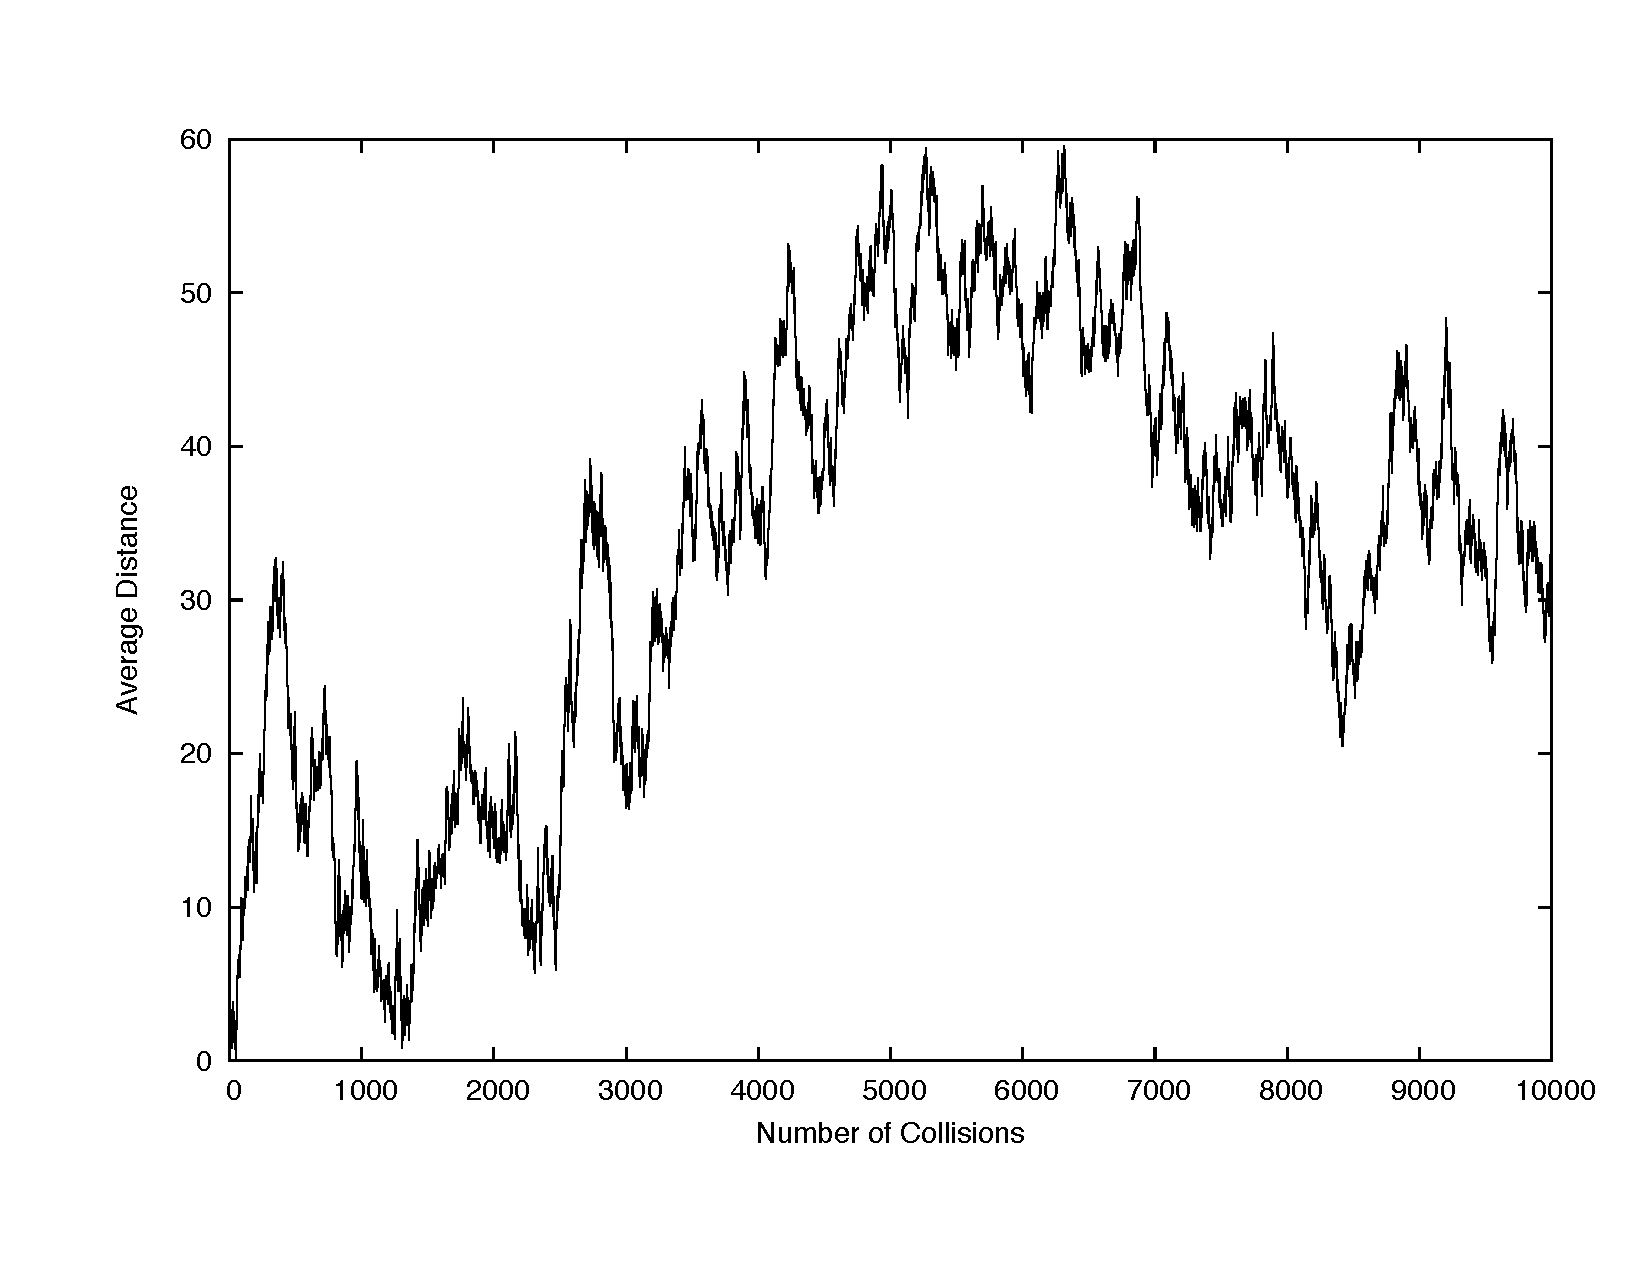
\includegraphics[width =120 mm, height = 90mm]{Ex_4_30_dist.pdf}
\caption{A plot of the average distance (Arb. Units) from the origin of the particle undergoing the random walk.}
\label{fig:RandomWalkDist}
\end{figure}
From Figures \ref{fig:RandomWalk} and \ref{fig:RandomWalkDist}, it is clear that the simulation creates the expected results.  The particle travels randomly in all directions and never strays more than 60 units from the origin.


\pagebreak
\section{Code}
\subsection{Exercise 12.10}
\begin{verbatim}
#include <stdio.h>
#include <stdlib.h>
#include <math.h>
#define pi 3.141592654
#define e  2.71828182845905

// Mitchell Miller
// PHYS 440 Lab 3
// Ex 12.10 2/28/12
// Monte Carlo Method

double sumRand(){

	double sum=0.;
	int counter;

	for(counter=0;counter<12;counter++){

		sum = sum + drand48();

	}

	return(sum);

}

int main(){

	int counter;
	double sum;

	FILE *outfile;
	outfile = fopen("Ex_12.10.dat","w");

	for(counter=0;counter<10000;counter++){

		sum = sumRand();
		fprintf(outfile,"%lf\n",sum);

	}

}
\end{verbatim}
\subsection{Exercise 4.4}
\begin{verbatim}
#include <stdio.h>
#include <stdlib.h>
#include <math.h>
#define pi 3.141592654

// Mitchell Miller
// PHYS 440 Lab 3
// Exc. 4.4 2/28/12
// Romberg Method

double func1(double x){

	// C(v) Fresnel Integral
	double funcValue;
	funcValue = cos(pi*x*x/2.);
	return(funcValue);

}

double func2(double x){

	// S(v) Fresnel Integral
	double funcValue;
	funcValue = sin(pi*x*x/2.);
	return(funcValue);

}

double romberg(double a, double b, int flag){

	double** t;
	int i,j,m,nMax;
	t = (double**) malloc(10*sizeof(double*));
	for(i=0;i<10;i++){
		t[i] = (double*) malloc(10*sizeof(double));
	}
	double sum,h;
	double a1,a2,a3,a4;
	double final;

	for(i=0;i<10;i++){
		for(j=0;j<10;j++){
			t[i][j] = 0;
		}
	}

	if(flag==0){
		t[0][0]=0.5*(b-a)*(func1(a)+func1(b));
	}
	else if(flag==1){
		t[0][0]=0.5*(b-a)*(func2(a)+func2(b));
	}
	
	for(m=0;m<9;m++){

		nMax = pow(2.,m+1) - 1;
		sum = 0;
		h = (b-a)/(pow(2,m+1));
		
		for(i=1;i<=nMax;i+=2){

			if(flag==0){

				sum = sum + func1(a+i*h);
		
			}
			else if(flag==1){

				sum = sum + func2(a+i*h);

			}

		}

		t[m+1][0] = 0.5 * t[m][0] + h*sum;

	}

	for(i=1;i<10;i++){

		for(j=1;j<=i;j++){

			if(j<=3){

				t[i][j] = (pow(4,j) * t[i][j-1] - t[i-1][j-1]) /  (pow(4,j)-1);

			}

		}

	}
/*
	for(i=0;i<10;i++){

		a1=t[i][0];
		a2=t[i][1];
		a3=t[i][2];
		a4=t[i][3];

		printf("%i\t%lf\t%lf\t%lf\t%lf\n",i,a1,a2,a3,a4);

	}*/
	
	final = t[9][3];
	return(final);

}

int main(){

	FILE *outfile;
	outfile = fopen("Ex_4.4.dat","w");

	double v,I;
	double C,S;
	int counter;

	v=0;

	for(counter=0;counter<1000;counter++){

		v = counter/100.;
		C = romberg(0,v,0);
		S = romberg(0,v,1);
		I = 0.5 * ( (C+0.5)*(C+0.5) + (S+0.5)*(S+0.5) );
		fprintf(outfile,"%lf\t%lf\n",v,I);

	}

}
\end{verbatim}
\subsection{Exercise 4.5}
\begin{verbatim}
#include <stdio.h>
#include <stdlib.h>
#include <math.h>
#define pi 3.14159265358979

// Mitchell Miller
// PHYS 440 Lab 3
// Exc. 4.4 2/28/12
// Romber Method

double func(double x){

	// Specify desired function
	double funcValue;
	funcValue = sin(x)*sin(x)*pow(2-cos(x),0.5);
	return(funcValue);

}

double main(){

	double** t;
	int i,j,m,nMax;
	t = (double**) malloc(10*sizeof(double*));
	for(i=0;i<10;i++){
		t[i] = (double*) malloc(10*sizeof(double));
	}
	double a,b,sum,h;
	double rm;
	double a1,a2,a3,a4;

	a = 0;
	b = pi;

	for(i=0;i<10;i++){
		for(j=0;j<10;j++){
			t[i][j] = 0;
		}
	}

	t[0][0]=0.5*(b-a)*(func(a)+func(b));
	
	for(m=0;m<9;m++){

		nMax = pow(2.,m+1) - 1;
		sum = 0;
		h = (b-a)/(pow(2,m+1));
		
		for(i=1;i<=nMax;i+=2){

			sum = sum + func(a+i*h);

		}

		t[m+1][0] = 0.5 * t[m][0] + h*sum;

	}

	for(i=1;i<10;i++){

		for(j=1;j<=i;j++){

			if(j<=3){

				t[i][j] = (pow(4,j) * t[i][j-1] - t[i-1][j-1]) /  (pow(4,j)-1);

			}

		}

	}

	for(i=0;i<10;i++){

		a1=t[i][0];
		a2=t[i][1];
		a3=t[i][2];
		a4=t[i][3];
		if(i>0&&i<9){

			rm = (t[i-1][0] - t[i][0]) / (t[i][0] - t[i+1][0]);
			if(t[i+1][0]==t[i][0]){
				rm=0;
			}

		}
		
		printf("%i\t%.15lf\t%.15lf\t%.15lf\t%.15lf\n",i,a1,a2,a3,a4,rm);

	}

}
\end{verbatim}
\begin{verbatim}
#include <stdio.h>
#include <stdlib.h>
#include <math.h>

// Mitchell Miller
// PHYS 440 Lab 3
// Exc. 4.4 2/28/12
// Romber Method

double func(double x){

	// Specify desired function
	double funcValue;
	funcValue = pow((1-x*x)*(2-x),0.5);
	return(funcValue);

}

double main(){

	double** t;
	int i,j,m,nMax;
	t = (double**) malloc(10*sizeof(double*));
	for(i=0;i<10;i++){
		t[i] = (double*) malloc(10*sizeof(double));
	}
	double a,b,sum,h;
	double rm;
	double a1,a2,a3,a4;

	a = -1.;
	b = 1.;

	for(i=0;i<10;i++){
		for(j=0;j<10;j++){
			t[i][j] = 0;
		}
	}

	t[0][0]=0.5*(b-a)*(func(a)+func(b));
	
	for(m=0;m<9;m++){

		nMax = pow(2.,m+1) - 1;
		sum = 0;
		h = (b-a)/(pow(2,m+1));
		
		for(i=1;i<=nMax;i+=2){

			sum = sum + func(a+i*h);

		}

		t[m+1][0] = 0.5 * t[m][0] + h*sum;

	}

	for(i=1;i<10;i++){

		for(j=1;j<=i;j++){

			if(j<=3){

				t[i][j] = (pow(4,j) * t[i][j-1] - t[i-1][j-1]) /  (pow(4,j)-1);

			}

		}

	}

	for(i=0;i<10;i++){

		a1=t[i][0];
		a2=t[i][1];
		a3=t[i][2];
		a4=t[i][3];
		if(i>0&&i<9){

			rm = (t[i-1][0] - t[i][0]) / (t[i][0] - t[i+1][0]);

		}
		
		printf("%i\t%lf\t%lf\t%lf\t%lf\t%lf\n",i,a1,a2,a3,a4,rm);

	}

}
\end{verbatim}
\subsection{Exercise 4.6}
\begin{verbatim}
#include <stdio.h>
#include <stdlib.h>
#include <math.h>
#define pi 3.141592654

// Mitchell Miller
// PHYS 440 Lab 3
// Exc. 4.6 2/28/12
// Romberg Method

double func(double theta, double x){

	// Period integration
	double funcValue;
	double length=1;
	double gravity=9.81;
	funcValue = 4.*pow(length/(gravity*(1-sin(theta/2)*sin(theta/2)*sin(x)*sin(x))),0.5);
	return(funcValue);

}

double romberg(double a, double b){

	double** t;
	double c = b;
	b = pi/2.0;
	int i,j,m,nMax;
	t = (double**) malloc(10*sizeof(double*));
	for(i=0;i<10;i++){
		t[i] = (double*) malloc(10*sizeof(double));
	}
	double sum,h;
	double a1,a2,a3,a4;
	double final;

	for(i=0;i<10;i++){
		for(j=0;j<10;j++){
			t[i][j] = 0;
		}
	}

	t[0][0]=0.5*(b-a)*(func(c,a)+func(c,b));
	
	for(m=0;m<9;m++){

		nMax = pow(2.,m+1) - 1;
		sum = 0;
		h = (b-a)/(pow(2,m+1));
		
		for(i=1;i<=nMax;i+=2){

			sum = sum + func(c,a+i*h);

		}

		t[m+1][0] = 0.5 * t[m][0] + h*sum;

	}

	for(i=1;i<10;i++){

		for(j=1;j<=i;j++){

			if(j<=3){

				t[i][j] = (pow(4,j) * t[i][j-1] - t[i-1][j-1]) /  (pow(4,j)-1);

			}

		}

	}
/*
	for(i=0;i<10;i++){

		a1=t[i][0];
		a2=t[i][1];
		a3=t[i][2];
		a4=t[i][3];

		printf("%i\t%lf\t%lf\t%lf\t%lf\n",i,a1,a2,a3,a4);

	}*/
	
	final = t[9][3];
	return(final);

}

int main(){

	FILE *outfile;
	outfile = fopen("Ex_4.6.dat","w");

	double theta0;
	double T,degrees;
	double Tactual = 2.00606668071065;
	double error;
	int counter;

	for(counter=0;counter<314;counter++){

		theta0 = counter/100.;
		degrees = theta0 * (180/pi);
		T = romberg(0,theta0);
		error = fabs((T-Tactual)/Tactual);
		fprintf(outfile,"%lf\t%lf\t%lf\n",degrees,T,error);

	}

}
\end{verbatim}
\subsection{Exercise 4.15}
\begin{verbatim}
#include <stdio.h>
#include <stdlib.h>
#include <math.h>
#define pi 3.141592654

// Mitchell Miller
// PHYS 440 Lab 3
// Exc. 4.15 2/28/12
// Gaussian Quadrature Method

double func(double x){

	double funcValue;
	funcValue = x*x*x*x*x*x*x;
	return(funcValue);

}

double map(double x){

	double mapValue;
	double a = 0;
	double b = 1;
	mapValue = (b-a)/2.*x + (a+b)/2.;
	return(mapValue);

}

double quad2(){

	double integral=0;
	int counter=0;
	int order=2;
	double x[2] = {0.5773502691896258,-0.5773502691896258};
	double w[2] = {1.0		 ,1.0		     };

	for(counter=0;counter<order;counter++){

		integral = integral + func(map(x[counter]))*w[counter];

	}
	
	integral = 0.5*integral;
	return(integral);

}

double quad3(){

	double integral=0;
	int counter=0;
	int order=3;
	double x[3] = {0.7745966692414834,0.0		    ,-0.7745966692414834};
	double w[3] = {0.5555555555555556,0.8888888888888889, 0.5555555555555556};

	for(counter=0;counter<order;counter++){

		integral = integral + func(map(x[counter]))*w[counter];

	}

	integral = 0.5*integral;
	return(integral);

}

double quad4(){

	double integral=0;
	int counter=0;
	int order=4;
	double x[4] = {0.8611363115940526,0.3399810435848563,-0.3399810435848563,-0.8611363115940526};
	double w[4] = {0.3478548451374539,0.6521451548625461, 0.6521451548625461, 0.3478548451374539};

	for(counter=0;counter<order;counter++){

		integral = integral + func(map(x[counter]))*w[counter];

	}

	integral = 0.5*integral;
	return(integral);

}

double quad5(){

	double integral=0;
	int counter=0;
	int order=5;
	double x[5] = {0.9061798459386640,0.5384693101056831,0.0	       ,-0.5384693101056831,-0.9061798459386640};
	double w[5] = {0.2369268850561891,0.4786286704993665,0.5688888888888889, 0.4786286704993665, 0.2369268850561891};

	for(counter=0;counter<order;counter++){

		integral = integral + func(map(x[counter]))*w[counter];

	}

	integral = 0.5*integral;
	return(integral);

}

int main(){

	double integral2,integral3,integral4,integral5;

	integral2 = quad2();
	integral3 = quad3();
	integral4 = quad4();
	integral5 = quad5();

	printf("N = 2\t%.15lf\n",integral2);
	printf("N = 3\t%.15lf\n",integral3);
	printf("N = 4\t%.15lf\n",integral4);
	printf("N = 5\t%.15lf\n",integral5);

}
\end{verbatim}
\subsection{Exercise 4.16}
\begin{verbatim}
#include <stdio.h>
#include <stdlib.h>
#include <math.h>
#define pi 3.141592654
#define e  2.71828182845905

// Mitchell Miller
// PHYS 440 Lab 3
// Exc. 4.16 2/28/12
// Gaussian Quadrature Method

double func(double x){

	double funcValue;
	funcValue = pow(e,-x*x);
	return(funcValue);

}

double map(double x){

	double mapValue;
	double a = 0;
	double b = 1;
	mapValue = (b-a)/2.*x + (a+b)/2.;
	return(mapValue);

}

double quad2(){

	double integral=0;
	int counter=0;
	int order=2;
	double x[2] = {0.5773502691896258,-0.5773502691896258};
	double w[2] = {1.0		 ,1.0		     };

	for(counter=0;counter<order;counter++){

		integral = integral + func(map(x[counter]))*w[counter];

	}
	
	integral = 0.5*integral;
	return(integral);

}

double quad3(){

	double integral=0;
	int counter=0;
	int order=3;
	double x[3] = {0.7745966692414834,0.0		    ,-0.7745966692414834};
	double w[3] = {0.5555555555555556,0.8888888888888889, 0.5555555555555556};

	for(counter=0;counter<order;counter++){

		integral = integral + func(map(x[counter]))*w[counter];

	}

	integral = 0.5*integral;
	return(integral);

}

double quad4(){

	double integral=0;
	int counter=0;
	int order=4;
	double x[4] = {0.8611363115940526,0.3399810435848563,-0.3399810435848563,-0.8611363115940526};
	double w[4] = {0.3478548451374539,0.6521451548625461, 0.6521451548625461, 0.3478548451374539};

	for(counter=0;counter<order;counter++){

		integral = integral + func(map(x[counter]))*w[counter];

	}

	integral = 0.5*integral;
	return(integral);

}

double quad5(){

	double integral=0;
	int counter=0;
	int order=5;
	double x[5] = {0.9061798459386640,0.5384693101056831,0.0	       ,-0.5384693101056831,-0.9061798459386640};
	double w[5] = {0.2369268850561891,0.4786286704993665,0.5688888888888889, 0.4786286704993665, 0.2369268850561891};

	for(counter=0;counter<order;counter++){

		integral = integral + func(map(x[counter]))*w[counter];

	}

	integral = 0.5*integral;
	return(integral);

}

int main(){

	double integral2,integral3,integral4,integral5;

	integral2 = quad2();
	integral3 = quad3();
	integral4 = quad4();
	integral5 = quad5();

	printf("N = 2\t%.15lf\n",integral2);
	printf("N = 3\t%.15lf\n",integral3);
	printf("N = 4\t%.15lf\n",integral4);
	printf("N = 5\t%.15lf\n",integral5);

}
\end{verbatim}
\subsection{Exercise 4.18}
\begin{verbatim}
#include <stdio.h>
#include <stdlib.h>
#include <math.h>
#define pi 3.141592654
#define e  2.71828182845905

// Mitchell Miller
// PHYS 440 Lab 3
// Exc. 4.18 2/28/12
// Gaussian Quadrature Method

double func(double x){

	double funcValue;
	funcValue = x*x*x/(1.-pow(e,-x));
	return(funcValue);

}

double map(double x){

	double mapValue;
	double a = 0;
	double b = 1;
	mapValue = (b-a)/2.*x + (a+b)/2.;
	return(mapValue);

}

double quad2(){

	double integral=0;
	int counter=0;
	int order=2;
	double x[2] = {5.8578643762690495e-1,3.4142135623730950   };
	double w[2] = {8.5355339059327376e-1,1.4644660940672624e-1};

	for(counter=0;counter<order;counter++){

		integral = integral + func(x[counter])*w[counter];

	}
	
	return(integral);

}

double quad4(){

	double integral=0;
	int counter=0;
	int order=4;
	double x[4] = {3.2254768961939231e-1,1.7457611011583466   ,4.5366202969211280   ,9.3950709123011331   };
	double w[4] = {6.0315410434163360e-1,3.5741869243779969e-1,3.8887908515005384e-2,5.3929470556132745e-4};

	for(counter=0;counter<order;counter++){

		integral = integral + func(x[counter])*w[counter];

	}

	return(integral);

}

double quad6(){

	double integral=0;
	int counter=0;
	int order=6;
	double x[6] = {2.2284660417926069e-1,1.1889321016726230   ,2.9927363260593141   ,5.7751435691045105   ,9.8374674183825899   ,1.5982873980601702e1 };
	double w[6] = {4.5896467394996359e-1,4.1700083077212099e-1,1.1337338207404498e-1,1.0399197453149075e-2,2.6101720281493206e-4,8.9854790642962124e-7};

	for(counter=0;counter<order;counter++){

		integral = integral + func(x[counter])*w[counter];

	}

	return(integral);

}

double quad8(){

	double integral=0;
	int counter=0;
	int order=8;
	double x[8] = {1.7027963230510100e-1,9.037017769937991e-1,2.2510866298661307   ,4.2667001702876588   ,7.0459054023934657   ,1.0758516010180995e1 ,1.5740678641278005e1 ,2.2863131736889296e1 };
	double w[8] = {3.6918858934163753e-1,4.1878678081434296e-1,1.7579498663717181e-1,3.3343492261215652e-2,2.7945362352256725e-3,9.0765087733582131e-5,8.4857467162725315e-7,1.0480011748715104e-9};

	for(counter=0;counter<order;counter++){

		integral = integral + func(x[counter])*w[counter];

	}

	return(integral);

}

int main(){

	double integral2,integral4,integral6,integral8;

	integral2 = quad2();
	integral4 = quad4();
	integral6 = quad6();
	integral8 = quad8();

	printf("N = 2\t%.15lf\n",integral2);
	printf("N = 4\t%.15lf\n",integral4);
	printf("N = 6\t%.15lf\n",integral6);
	printf("N = 8\t%.15lf\n",integral8);

}
\end{verbatim}
\subsection{Exercise 4.19}
\begin{verbatim}
#include <stdio.h>
#include <stdlib.h>
#include <math.h>
#define pi 3.141592654
#define e  2.71828182845905

// Mitchell Miller
// PHYS 440 Lab 3
// Exc. 4.19 2/28/12
// Gaussian Quadrature Method

double func(double x, double y){

	double funcValue;
	funcValue = pow(e,-x*y);
	return(funcValue);

}

double mapX(double x){

	double mapValue;
	double a = 0;
	double b = 2;
	mapValue = (b-a)/2.*x + (a+b)/2.;
	return(mapValue);

}

double mapY(double y){

	double mapValue;
	double a = 0;
	double b = 1;
	mapValue = (b-a)/2.*y + (a+b)/2.;
	return(mapValue);

}


double FofY(double y){

	double integral=0;
	int counter=0;
	int order=5;
	double x[5] = {0.9061798459386640,0.5384693101056831,0.0	       ,-0.5384693101056831,-0.9061798459386640};
	double w[5] = {0.2369268850561891,0.4786286704993665,0.5688888888888889, 0.4786286704993665, 0.2369268850561891};

	for(counter=0;counter<order;counter++){

		integral = integral + func(mapX(x[counter]),mapY(y))*w[counter];

	}

	integral = 0.5*integral;
	return(integral);

}

double quad5(){

	double integral=0;
	int counter=0;
	int order=5;
	double x[5] = {0.9061798459386640,0.5384693101056831,0.0	       ,-0.5384693101056831,-0.9061798459386640};
	double w[5] = {0.2369268850561891,0.4786286704993665,0.5688888888888889, 0.4786286704993665, 0.2369268850561891};

	for(counter=0;counter<order;counter++){

		integral = integral + FofY(x[counter])*w[counter];

	}

	return(integral);

}


int main(){

	double integral2,integral3,integral4,integral5;

	integral5 = quad5();

	printf("N = 5\t%.15lf\n",integral5);

}
\end{verbatim}
\subsection{Exercise 4.22}
\begin{verbatim}
#include <stdio.h>
#include <stdlib.h>
#include <math.h>
#define pi 3.141592654
#define e  2.71828182845905

// Mitchell Miller
// PHYS 440 Lab 3
// Exc. 4.22 2/28/12
// Gaussian Quadrature Method

double func(double x, double y, double xp, double yp){

	double funcValue;
	funcValue = pow((x-xp)*(x-xp)+(y-yp)*(y-yp),-0.5);
	return(funcValue);

}

double mapX(double x){

	double mapValue;
	double a = 0;
	double b = 2;
	mapValue = (b-a)/2.*x + (a+b)/2.;
	return(mapValue);

}

double mapY(double y){

	double mapValue;
	double a = 0;
	double b = 1;
	mapValue = (b-a)/2.*y + (a+b)/2.;
	return(mapValue);

}


double FofY(double y, double xp, double yp){

	double integral=0;
	int counter=0;
	int order=5;
	double x[5] = {0.9061798459386640,0.5384693101056831,0.0	       ,-0.5384693101056831,-0.9061798459386640};
	double w[5] = {0.2369268850561891,0.4786286704993665,0.5688888888888889, 0.4786286704993665, 0.2369268850561891};

	for(counter=0;counter<order;counter++){

		integral = integral + func(x[counter],y,xp,yp)*w[counter];

	}

	return(integral);

}

double quad5(double xp, double yp){

	double integral=0;
	int counter=0;
	int order=5;
	double x[5] = {0.9061798459386640,0.5384693101056831,0.0	       ,-0.5384693101056831,-0.9061798459386640};
	double w[5] = {0.2369268850561891,0.4786286704993665,0.5688888888888889, 0.4786286704993665, 0.2369268850561891};

	for(counter=0;counter<order;counter++){

		integral = integral + FofY(x[counter],xp,yp)*w[counter];

	}

	return(integral);

}


int main(){

	FILE *outfile;
	outfile = fopen("Ex_4.22.dat","w");

	double integral2,integral3,integral4,integral5;
	int xp,yp;

	for(xp=2;xp<21;xp+=2){

		for(yp=2;yp<21;yp+=2){

			integral5 = quad5(xp,yp);

			fprintf(outfile,"%i\t%i\t%lf\n",xp,yp,integral5);

		}

	}

}
\end{verbatim}
\subsection{Exercise 4.30}
\begin{verbatim}
#include <stdio.h>
#include <stdlib.h>
#include <math.h>
#define pi 3.141592654
#define e  2.71828182845905

// Mitchell Miller
// PHYS 440 Lab 3
// Exc. 4.30 2/28/12
// Random Walk Simulation

int main(){

	double timeStep;
	int counter=0,steps;
	double x,y,z;
	double vx,vy,vz,v0;
	double theta,phi;
	double distance;

	FILE *outfile;
	outfile = fopen("Ex_4.30.dat","w");

	theta = pi * drand48();
	phi = 2.0 * pi * drand48();
	v0 = 10;

	vx = v0 * sin(theta) * cos(phi);
	vy = v0 * sin(theta) * sin(phi);
	vz = v0 * cos(theta);
	x = 0;
	y = 0;
	z = 0;
	distance = sqrt(x*x+y*y+z*z);

	timeStep = 0.1;
	steps = 10000;

	fprintf(outfile,"%i\t%lf\n",counter,distance);

	for(counter=0;counter<steps;counter++){

		x = x + vx*timeStep;
		y = y + vy*timeStep;
		z = z + vz*timeStep;
		distance = sqrt(x*x+y*y+z*z);

		fprintf(outfile,"%i\t%lf\n",counter,distance);

		theta = pi * drand48();
		phi = 2.0 * pi * drand48();

		vx = v0 * sin(theta) * cos(phi);
		vy = v0 * sin(theta) * sin(phi);
		vz = v0 * cos(theta);

	}

}
\end{verbatim}
\begin{verbatim}
#include <stdio.h>
#include <stdlib.h>
#include <math.h>
#define pi 3.141592654
#define e  2.71828182845905

// Mitchell Miller
// PHYS 440 Lab 3
// Exc. 4.30 2/28/12
// Random Walk Simulation

typedef struct{
	double a;
	double b;
	double c;
} point;

void step(point * pos, point * vel, double t){

	(*pos).a = (*pos).a + (*vel).a*t;
	(*pos).b = (*pos).b + (*vel).b*t;
	(*pos).c = (*pos).c + (*vel).c*t;

}

void randVeloc(point * vel){

	double theta,phi;
	double v0 = 10;	

	theta = pi * drand48();
	phi = 2.0 * pi * drand48();

	(*vel).a = v0 * sin(theta) * cos(phi);
	(*vel).b = v0 * sin(theta) * sin(phi);
	(*vel).c = v0 * cos(theta);

}

int main(){

	struct point {
		double a;
		double b;
		double c;
	} my_point;

	struct point *position = &my_point;
	struct point *velocity = &my_point;
	double timeStep, distance;
	int counter,steps;

	FILE *outfile;
	outfile = fopen("Ex_4.30.dat","w");

	randVeloc(velocity);

	timeStep = 0.1;
	counter=0;
	steps = 10000;
	distance = sqrt((*position).a*(*position).a + (*position).b*(*position).b + (*position).c*(*position).c);

	fprintf(outfile,"%i\t%lf\n",counter,distance);

	for(counter=0;counter<steps;counter++){

		step(position,velocity,timeStep);

		distance = sqrt((*position).a*(*position).a + (*position).b*(*position).b + (*position).c*(*position).c);

		fprintf(outfile,"%i\t%lf\n",counter,distance);

		randVeloc(velocity);

	}

}
\end{verbatim}
\subsection{Figure 4.12}
\begin{verbatim}
#include <stdio.h>
#include <stdlib.h>
#include <math.h>
#define pi 3.141592654
#define e  2.71828182845905

// Mitchell Miller
// PHYS 440 Lab 3
// Fig 4.12 2/28/12
// Monte Carlo Method

double func(double x){

	double funcValue;
	funcValue = pow(e,x);
	return(funcValue);

}

double monteCarlo(){

	double sum=0.;
	int counter1,counter2;
	double N;
	double monte,x,error;

	for(counter1=1;counter1<401;counter1++){

		for(counter2=1;counter2<11;counter2++){

			x = drand48();
			sum = sum + func(x);

		}

		N = counter1 * 10.;

		monte = sum/N;

		error = fabs(monte - (e-1.))/(e-1.);

		//printf("N = %lf\t%lf\t%lf\n",N,monte,error);

	}

	return(monte);

}	

int main(){

	FILE *outfile;
	outfile = fopen("Fig_4.12.400.dat","w");
	double integral;
	int counter;
	
	for(counter=0;counter<10000;counter++){
	
		integral = monteCarlo();
		fprintf(outfile,"%lf\n",integral);
		
	}

}	
\end{verbatim}
\subsection{Helium Atom}
\begin{verbatim}
//
//  main.c
//  HeAtom
//
//  Created by Mitchell Miller on 3/23/12.
//  Copyright 2012 __MyCompanyName__. All rights reserved.
//

#include <math.h>
#include <stdio.h>
#include <stdlib.h>
#include <time.h>

double bohrRadius = .5291772083; //angstroms
double Pi = 3.141592653589793;
double E = 2.718281828459045;
double eCharge = 14.39964439;
double Z = 2;
int numberOfLoops = 10000000;

double oneSState(double x,double y,double z){
    
    double funcValue;
    double exp = 0;
    double radius = sqrt(x*x+y*y+z*z);
    
    exp = -2*Z*radius/bohrRadius;
    funcValue = pow(E,exp);
    
    return(funcValue);
    
}

double twoSState(double x,double y,double z){
    
    double funcValue;
    double exp;
    double coef;
    double expTerm;
    
    double radius = sqrt(x*x+y*y+z*z);
    
    coef = pow(1. - 0.5*Z*radius/bohrRadius,2);
    exp = -Z*radius/bohrRadius;
    expTerm = pow(E,exp);
    funcValue = coef*expTerm;
    
    return(funcValue);
}

double twoPState(double x,double y,double z){
    
    double funcValue;
    double exp;
    double coef;
    double expTerm;
    
    double radius = sqrt(x*x+y*y+z*z);
    
    exp = -2*Z*radius/bohrRadius;
    coef = radius*radius;
    expTerm = pow(E,exp);
    funcValue = coef*expTerm;
    
    return(funcValue);
}

double K1s2sIntegral(double x1,double y1,double z1,double x2,double y2,double z2){
    
    double funcValue;
    double coef;
    double exp;
    double radius1 = sqrt(x1*x1+y1*y1+z1*z1);
    double radius2 = sqrt(x2*x2+y2*y2+z2*z2);
    
    coef = (1-(.5)*Z*radius2/bohrRadius)*(1-(.5)*Z*radius1/bohrRadius);
    exp = -Z*(radius1+radius2)* (3/ (2*bohrRadius));
    funcValue = coef*pow(E,exp);
    
    return(funcValue);
}

double K1s2pR(double x,double y,double z){
    
    double funcValue;
    double exp;
    
    double radius = sqrt(x*x+y*y+z*z);
    exp = -(3*Z*radius/(2*bohrRadius));
    funcValue = z*pow(E,exp);
    
    return(funcValue);
}

double repulsion(double x1,double y1,double z1,double x2,double y2,double z2){
    
    double funcValue;
    double radius = sqrt((x1-x2)*(x1-x2)+(y1-y2)*(y1-y2)+(z1-z2)*(z1-z2));
    
    funcValue = 1 / fabs(radius);
    
    return(funcValue);
}

double J1S2S(double low, double high){
    
    double funcValue=0;
    int counter;
    
    double x1=0;
    double x2=0;
    double y1=0;
    double y2=0;
    double z1=0;
    double z2=0;
    
    double oneS=0;
    double twoS=0;
    double repul=0;
    
    double width = high - low;
    
    double coef1S = pow((Z / bohrRadius),3) / Pi;
    double coef2S = pow((Z / bohrRadius),3) / (8*Pi);
    
    for(counter=0;counter<numberOfLoops;counter++){
        
        x1 = (drand48() - 0.5) * width;
        y1 = (drand48() - 0.5) * width;
        z1 = (drand48() - 0.5) * width;
        x2 = (drand48() - 0.5) * width;
        y2 = (drand48() - 0.5) * width;
        z2 = (drand48() - 0.5) * width;
        
        oneS = fabs(oneSState(x1, y1, z1));
        twoS = fabs(twoSState(x2, y2, z2));
        repul = repulsion(x1, y1, z1, x2, y2, z2);
        
        funcValue += oneS * twoS * repul;
        
    }
    
    funcValue /= numberOfLoops;
    funcValue *= coef1S*coef2S*eCharge*pow(width,6);
    return(funcValue);
    
}

double K1S2S(double low, double high){
    
    double funcValue=0;
    int counter;
    
    double x1=0;
    double x2=0;
    double y1=0;
    double y2=0;
    double z1=0;
    double z2=0;
    
    double repul;
    double kInteg;
    double zBohr = Z / bohrRadius;
    double coef1S = (1 / (8*pow(Pi,2)))*pow(zBohr,6);
    
    double width = high - low;
    
    
    for(counter=0;counter<numberOfLoops;counter++){
        
        x1 = (drand48() - 0.5) * width;
        y1 = (drand48() - 0.5) * width;
        z1 = (drand48() - 0.5) * width;
        x2 = (drand48() - 0.5) * width;
        y2 = (drand48() - 0.5) * width;
        z2 = (drand48() - 0.5) * width;
        
        kInteg = K1s2sIntegral(x1,y1,z1,x2,y2,z2);
        repul = repulsion(x1, y1, z1, x2, y2, z2);
        funcValue += kInteg*repul;
        
    }
    
    funcValue = funcValue / numberOfLoops;
    funcValue = funcValue * eCharge*pow(width,6)*coef1S;
    return(funcValue);
    
}

double J1S2P(double low, double high){
    
    double funcValue=0;
    int counter;
    double width = high - low;
    
    double x1=0;
    double x2=0;
    double y1=0;
    double y2=0;
    double z1=0;
    double z2=0;
    
    double zBohr = Z / bohrRadius;
    double repul=0;
    double oneS=0;
    double twoP=0;
    
    double coef1S = pow(zBohr,3) / Pi;
    double coef2P = (1 / (64*pow(Pi,2)))*pow(zBohr,8);
    
    for(counter=0;counter<numberOfLoops;counter++){
        
        x1 = (drand48() - 0.5) * width;
        y1 = (drand48() - 0.5) * width;
        z1 = (drand48() - 0.5) * width;
        x2 = (drand48() - 0.5) * width;
        y2 = (drand48() - 0.5) * width;
        z2 = (drand48() - 0.5) * width;
     
        oneS = oneSState(x1, y1, z1);
        twoP = twoPState(x2, y2, z2);
        repul = repulsion(x1, y1, z1, x2, y2, z2);
        
        funcValue += oneS*twoP*repul;
        
    }
    
    funcValue = funcValue / numberOfLoops;
    funcValue = funcValue * coef1S*coef2P*eCharge*pow(width,6);    // May need to add 'coef1S' here
    
    return(funcValue);
}

double K1S2P(double low, double high){
    
    double funcValue=0;
    int counter;
    double width = high - low;
    
    double x1=0;
    double x2=0;
    double y1=0;
    double y2=0;
    double z1=0;
    double z2=0;
    
    double zBohr = Z / bohrRadius;
    double repul;
    double r1;
    double r2;
    double coef2P = (1 / (32*pow(Pi,2)))*pow(zBohr,8);

    for(counter=0;counter<numberOfLoops;counter++){
        
        x1 = (drand48() - 0.5) * width;
        y1 = (drand48() - 0.5) * width;
        z1 = (drand48() - 0.5) * width;
        x2 = (drand48() - 0.5) * width;
        y2 = (drand48() - 0.5) * width;
        z2 = (drand48() - 0.5) * width;
        
        r1 = K1s2pR(x1, y1, z1);
        r2 = K1s2pR(x2, y2, z2);
        repul = repulsion(x1, y1, z1, x2, y2, z2);
        
        funcValue += r1*r2*repul;
        
    }
    
    funcValue = funcValue / numberOfLoops;
    funcValue = funcValue * eCharge*pow(width,6)*coef2P;
    
    return(funcValue);
    
}

int main ()
{

    double lower = -5;
    double upper = 5;
    double j1s2s=0;
    double k1s2s=0;
    double j1s2p=0;
    double k1s2p=0;
    
    int counter;
    int loops=1000;
    
    FILE *outfile;
    outfile = fopen("HeAtom.dat","w");
    
    srand48( time(NULL));
    
    for(counter=0;counter<loops;counter++){
        
        printf("Begin Loop\t");
        j1s2s += J1S2S(lower, upper);
        j1s2p += J1S2P(lower, upper);
        
        k1s2s += K1S2S(lower, upper);
        k1s2p += K1S2P(lower, upper);
        
        printf("Loop %i Complete\n",counter);
        
    }
    
    j1s2s = j1s2s / loops;
    j1s2p = j1s2p / loops;
    k1s2s = k1s2s / loops;
    k1s2p = k1s2p / loops;
    
    printf("J1S2S = %lf\n",j1s2s);
    printf("K1S2S = %lf\n",k1s2s);
    printf("J1S2P = %lf\n",j1s2p);
    printf("K1S2P = %lf\n",k1s2p);
    
    fclose(outfile);
    
    return 0;
}
\end{verbatim}


\end{document}

